\documentclass{standalone}
\usepackage{graphicx}	
\usepackage{amssymb, amsmath}
\usepackage{color}

\usepackage{tikz}
\usetikzlibrary{intersections, backgrounds}

\definecolor{light}{RGB}{220, 188, 188}
\definecolor{mid}{RGB}{185, 124, 124}
\definecolor{dark}{RGB}{143, 39, 39}
\definecolor{highlight}{RGB}{180, 31, 180}
\definecolor{gray10}{gray}{0.1}
\definecolor{gray20}{gray}{0.2}
\definecolor{gray30}{gray}{0.3}
\definecolor{gray40}{gray}{0.4}
\definecolor{gray60}{gray}{0.6}
\definecolor{gray70}{gray}{0.7}
\definecolor{gray80}{gray}{0.8}
\definecolor{gray90}{gray}{0.9}
\definecolor{gray95}{gray}{0.95}

\newcommand*{\offset}{0.025}

\begin{document}

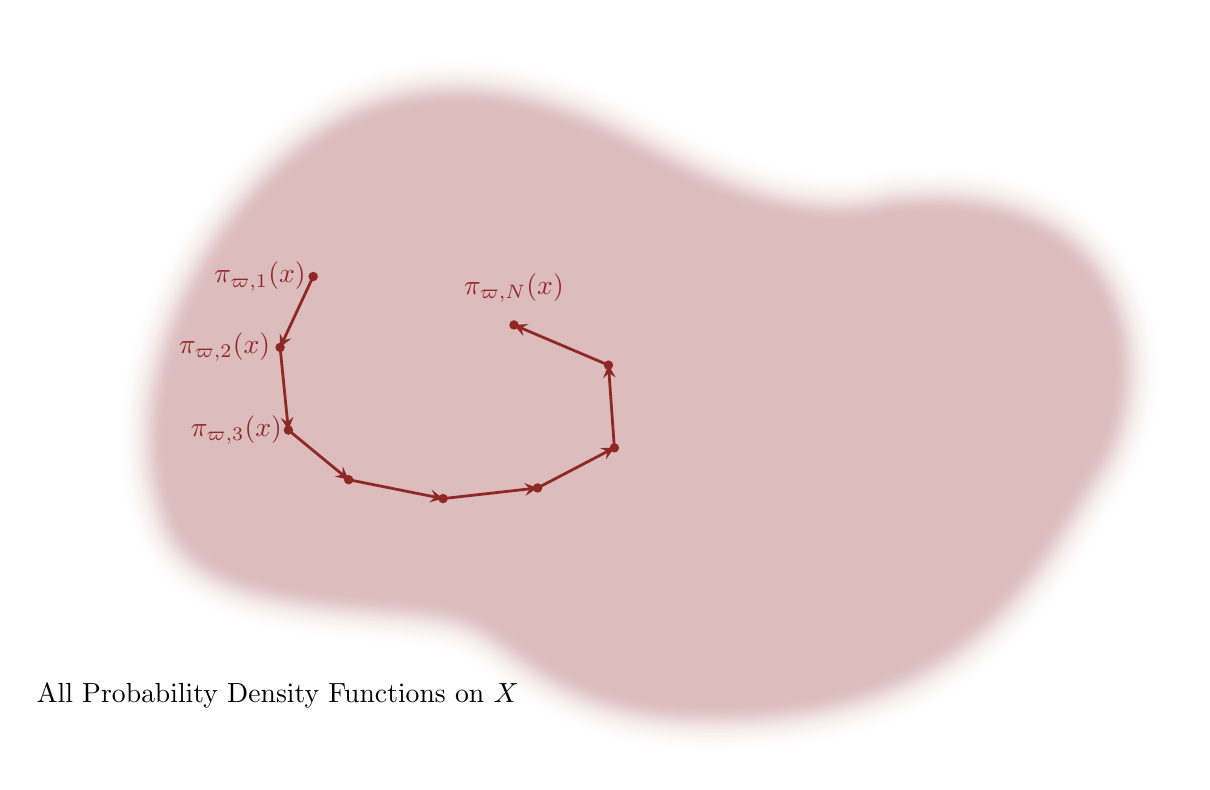
\begin{tikzpicture}[scale=0.3, thick]               
 \pgfmathsetmacro{\dx}{18}
 
 \foreach \i in {0.025, 0.05, ..., 1} {
   \draw[line width={40 * \i}, opacity={exp(-5 * \i))}, light] 
     (-20, -2)
    .. controls (-22, 4) and (-17, 12) .. (-12, 14)  
    .. controls (-7, 16) and (-2, 13) .. (0, 12)
    .. controls (2, 11) and (6, 9) .. (10, 10)
    .. controls (20, 11) and (20, 3) .. (18, 0)
    .. controls (15.5, -4) and (13, -9.5) .. (4, -10)
    .. controls (-4, -10.5) and (-5, -7) .. (-8, -6)
    .. controls (-11, -5) and (-19, -6) .. (-20, -2);
  }
  
  \fill [fill=light] (-20, -2)
    .. controls (-22, 4) and (-17, 12) .. (-12, 14)  
    .. controls (-7, 16) and (-2, 13) .. (0, 12)
    .. controls (2, 11) and (6, 9) .. (10, 10)
    .. controls (20, 11) and (20, 3) .. (18, 0)
    .. controls (15.5, -4) and (13, -9.5) .. (4, -10)
    .. controls (-4, -10.5) and (-5, -7) .. (-8, -6)
    .. controls (-11, -5) and (-19, -6) .. (-20, -2);
    
  \node [] at (-16, -10) { All Probability Density Functions on $X$ };
      
  %\draw [color=dark] (-14.5, 7.75) 
  %  .. controls (-16, 5) and (-17.5, 2.75) .. (-14.5, 0)
  %  .. controls (-11.5, -2.75) and (-5, -1.5) .. (-3, -0.5)
  %  .. controls (-1, 0.5) and (-0.5, 3) .. (-2.5, 4.5)
  %  .. controls (-4.5, 6) and (-7, 6) .. (-9, 5)
  %  .. controls (-11, 4) and (-11, 2) .. (-9, 1)
  %  .. controls (-7, 0) and (-5, 0) .. (-3, 1);
  
  \node [color=dark] at (-16.75, 7.75) { $\pi_{\varpi, 1}(x)$ };
  \fill[dark] (-14.5, 7.75) circle (0.2);
  
  \draw[->, >=stealth, line width=1, color=dark] (-14.5, 7.75) -- (-15.9, 4.75);
  
  \node [color=dark] at (-18.25, 4.75) { $\pi_{\varpi, 2}(x)$ };
  \fill[dark] (-15.9, 4.75) circle (0.2);
  
  \draw[->, >=stealth, line width=1, color=dark] (-15.9, 4.75) -- (-15.55, 1.25);
  
  \node [color=dark] at (-17.75, 1.25) { $\pi_{\varpi, 3}(x)$ };
  \fill[dark] (-15.55, 1.25) circle (0.2);
  
  \draw[->, >=stealth, line width=1, color=dark] (-15.55, 1.25) -- (-13, -0.85);
  
  \fill[dark] (-13, -0.85) circle (0.2);
  
  \draw[->, >=stealth, line width=1, color=dark] (-13, -0.85) -- (-9, -1.65);
  
  \fill[dark] (-9, -1.65) circle (0.2);
  
  \draw[->, >=stealth, line width=1, color=dark] (-9, -1.65) -- (-5, -1.2);
  
  \fill[dark] (-5, -1.2) circle (0.2);
  
  \draw[->, >=stealth, line width=1, color=dark] (-5, -1.2) -- (-1.75, 0.5);
  
  \fill[dark] (-1.75, 0.5) circle (0.2);
  
  \draw[->, >=stealth, line width=1, color=dark] (-1.75, 0.5) -- (-2, 4);
  
  \fill[dark] (-2, 4) circle (0.2);
  
  \draw[->, >=stealth, line width=1, color=dark] (-2, 4) -- (-6, 5.7);
  
  \node [color=dark] at (-6, 7.25) { $\pi_{\varpi, N}(x)$ };
  \fill[dark] (-6, 5.7) circle (0.2);

\end{tikzpicture}

\end{document}   